\newcommand{\package}{\emph}

\setcounter{chapter}{1}
\setcounter{section}{0}
\section{Problem 1: Logistic difference equation}
\subsection{a: Finding the equilibrium points}
We can find equilibrium points from  
\begin{equation}
f(x, a) = ax(1-x) = x
\label{eq:p01_main}
\end{equation}
as the roots of the quadratic equation:
\begin{equation}
ax^2 - (a - 1)x = x(ax - (a - 1)) = 0
\end{equation}
which are:
\begin{align}
x^*_1 &= 0 \\
x^*_2 &= \frac{(a-1)}{a}
\end{align}
The fixed point $x_2$ is non-negative if $a \geq 1$.
One can analyze the local stability of the difference equation \ref{eq:p01_main} by examining the partial derivative of $f$ with respect to $x$ evaluated at each fixed point $x^{\ast}$:
\begin{equation}
f' = - ax - a(x - 1) = a- 2ax
\label{eq:p01_diffmain}
\end{equation}

For $|f'_{x} | < 1$ the equlibrium point is attractive.

\[x^*_1 = 0 \rightarrow f'_{(x)} = a -2a(0) = a \rightarrow |a| < 1 \text{ then } x^*_1 \text{ is attractive}\]
\[x^*_2 = \frac{(a-1)}{a} \rightarrow f'_{(x)} = a -2a +2 = -a+2 \rightarrow |2-a| < 1 \text{ for } 1<a<3 \text{ then }x^*_1 \text{ is attractive}\]

\subsection{b: Point stability at different values of $a$}

When \textbf{$a = 0.9$}
\begin{eqnarray}
x^*_1 = 0 \rightarrow |a| = |0.9| < 1 \textbf{ attractive}\\
x^*_2 = \frac{(a-1)}{a}  \rightarrow |2-0.9|  = |1.1| > 1 \textbf{ not attractive}\\
\end{eqnarray}
When \textbf{$a = 2.1$}
\begin{eqnarray}
x^*_1 = 0 \rightarrow |a| = |2.1| > 1 \textbf{ not attractive}\\
x^*_2 = \frac{(a-1)}{a}  \rightarrow |2-2.1|  = |0.1| < 1 \textbf{ attractive}\\
\end{eqnarray}

When \textbf{$a = 3..58$} 
\begin{eqnarray}
x^*_1 = 0 \rightarrow |a| = |3.58| > 1 \textbf{ not attractive}\\
x^*_2 = \frac{(a-1)}{a}  \rightarrow |2-3.58|  = |1.58| > 1 \textbf{ not attractive}\\
\end{eqnarray}

In a conceptual view we can see for $a$ values in excess of $3.57$, the orbits $x(t, x0) = {x0, x1, x2, ... }$ depend crucially on the initial condition $x0$. Slight variations in $x0$ result in dramatically different orbits, an important characteristic of chaos.

\begin{figure}[h]
 \centering
    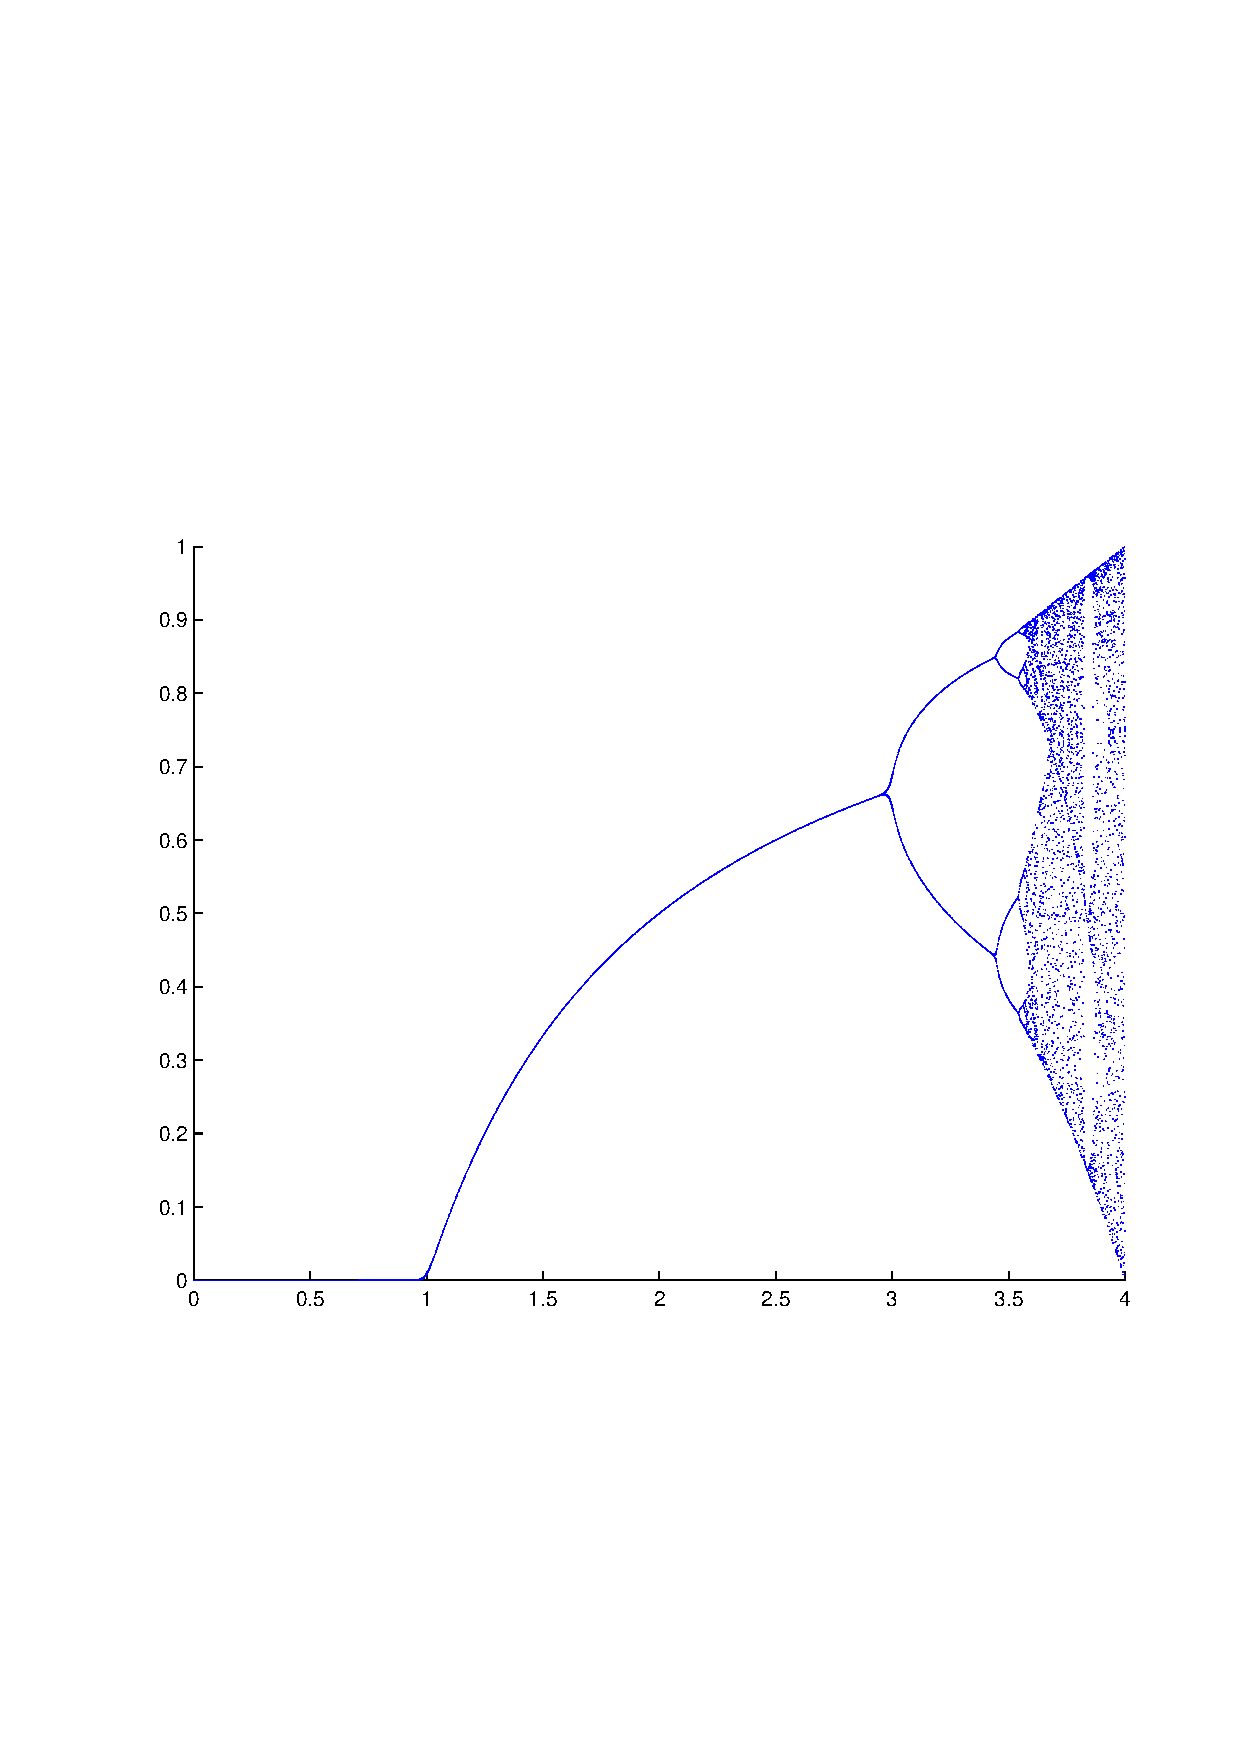
\includegraphics[scale=0.55]{plot_A01_P01.pdf}
    \caption{Logistic Map Bifurcation Diagram}
	\label{fig:plot_logistic_map_bifgraph}
\end{figure}


\setcounter{chapter}{2}
\setcounter{section}{0}
\section{Problem 2: Logistic growth in continuous time}
\subsection{a: Finding solution of logistic equation}
We have to solve the equation
\begin{equation}
\frac{dx}{dt} = rx (1-\frac{x}{K})  = r(x - \frac{x^2}{K}) = \frac{rx(K-x)}{K}
\label{eq:p02_main}
\end{equation}
using the separation of variables
\begin{equation}
\frac{K}{x(K-x)}dx = rdt
\end{equation}
decomposing the right part with partial fractions
\begin{equation}
\frac{K}{x(K-x)}=\frac{A}{x} + \frac{B}{K-x}
\end{equation}
We find A and B
\begin{align}
A&= \frac{K - Bx}{K-x} \\
B &= \frac{K-A(K-x)}{x}
\end{align}
Supposing $A = 1$, and according to above, $B$ is also equal to $1$, so our partial fraction decomposition is
\begin{equation}
\frac{K}{x(K-x)}=\frac{1}{x} + \frac{1}{K-x}
\end{equation}
Now we have to take the integral from both parts:
\begin{align}
\int{\frac{1}{x}+\frac{1}{K-x}dx} &= \int{rdt}\\
\int{\frac{1}{x}}+\int{\frac{1}{K-x}dx} &= r\int{dt}\\
\ln{x} - \ln{K-x} &= rt + x_0\\
\ln{\frac{x}{K-x}} &= rt + x_0\\
\frac{x}{K-x} &= x_0e^{rt}
\end{align}
Finally the solution 
\begin{equation}
x(t) = x_0Ke^{rt}\frac{1}{K + x_0(e^{rt}-1)}
\end{equation}

To prove it we explict the computation behind our results$ (\lambda = r)$:

\[\frac{dx}{dt} = \lambda x (1-\frac{x}{k}) = \lambda x (\frac{k-x}{k}) \rightarrow \int \frac{k}{x(k-x)}dx = \int \lambda dt \]
\[ \int [ \frac{1}{x} + \frac{1}{k-x}]dx = \int \lambda dt \rightarrow \ln |x| - \ln |k-x| = \lambda t + c \rightarrow \]
\[ \rightarrow \ln |k-x| - \ln |x| = -\lambda t - x \rightarrow \ln | \frac{k-x}{x} | = e^{-\lambda t -c} = \frac{k-x}{x} = \pm e^{-\lambda t}e^{-c} \text{ with } A = e^{-c} \]
\[ \rightarrow \frac{k-x}{x} = Ae^{-\lambda t} = \frac{k}{x} -1 = Ae^{-\lambda t} \rightarrow x = \frac{k}{1+Ae^{-\lambda t}} = \frac{k}{1+Ae^{-\lambda t}}(\frac{e^{\lambda t}}{e^{\lambda t}}) = \frac{ke^{\lambda t}}{e^{\lambda t}+A} \]

\[ x_0 = x(0) = \frac{k}{1+A} = x_0 \rightarrow k = x_0 + Ax_0 = k-x_0 = Ax_0 \rightarrow A = \frac{k-x_0}{x_0} \]

\[ x = \frac{ke^{\lambda t}}{e^{\lambda t} + \frac{k-x_0}{x_0}} = \frac{kx_0e^{\lambda t}}{e^{\lambda t}x_0+k-x_0} = \frac{kx_0e^{\lambda t}}{k+x_0(e^{\lambda t} -1)} \]




\subsection{b: Determining the stability of equilibrium points}

To determine the stability of the two equilibria points found solving the equation \ref{eq:p02_main} in $0$
\begin{align}
x^*_1 &= 0\\
x^*_2 &= K
\end{align}
one has to derive it for $x$:
\begin{equation}
f'(x) = - r(\frac{x}{K} - 1) - \frac{rx}{K}\\
\label{eq:p02_diffmain}
\end{equation}
Substituting $x^*_1$ and $x^*_2$ into \ref{eq:p02_diffmain} yields:
\begin{align}
f'(x^*_1) &= r \text{ if } r < 0 \textbf{ stable equilibrium}\\
f'(x^*_2) &= -r \text{ if } r > 0 \textbf{ stable equilibrium}
\end{align}

One finds that if $ f'(x_1) $ with $x_1 = 0$, then $x^{\ast}$ is always stable, while if $ for r < 0 \rightarrow f'(x_2) > 0 $ with $x_2 = -r $ $x^{\ast}$ is repelling.



\setcounter{chapter}{3}
\setcounter{section}{0}
\section{Problem 3: Hardy-Weinberg equilibrium}
\subsection{a: frequency of allele B in population}
Assuming HWE fot three alleles (allele and genotype frequences):

\[  (A+B+0)^2 = A^2 + B^2 + 0^2 + 2AB + 2A0 + 2B0 = 1  \]

We could solve the equation: 

\[  (A+B+0)^2 = (p+q+r)^2 = p^2 + q^2 + r^2 + 2pq + 2pr + 2qr = 1  \]

And given observable genotype frequences
\begin{align}
0^2 &= \frac{900}{10000} = 0.09 = r^2 \rightarrow r = 0.3 \\
2AB &= \frac{2000}{10000} = 0.20 = 2pq \rightarrow pq = 0.1 \\
A^2 + 2A0 &= \frac{1600}{10000} = 0.16 = p^2 + 2pr\\
\\
p^2+2*0.3*p &= 0.16 \\
p_1 &= \frac{1}{5} \\
p_2 &= -\frac{4}{5} \text{~not acceptable}\\
\\
q = \frac{0.1}{0.2} = 0.5
\end{align}

So, the frequency for $B$ allele is equal to $0.5$

\subsection{b: HW Equilibrium}
The equilibrium is given by $p^* = P^2+pq+pr$
\begin{align}
A^2 &= \frac{1500}{10000} = 0.15 = p^2 \rightarrow p = 0.39 \\
p^2+2pr &= \frac{1600}{10000} = 0.16 \rightarrow 0.15+2pr = 0.16 \rightarrow pr = \frac{0.01}{2} = 0.005\\
2pq &= \frac{2000}{10000} = 0.2 \rightarrow pq = 0.1\\
\end{align}

\[ p^* = 0.15+0.0005 + 0.1 = 0.255 \]

So, for the next round of random mating, the number of genotype $AA = (P^*)^2 * 10000 = (0.255)^2*10000 = 650 \neq 1500$.
The first generation is not in Hardy-Weinberg equilibrium.

Hence, assuming population carrying $AA$ is $1500$, we are not at the equilibrium of HW $(p^{2}_b = 0.15 \neq p^{2}_a = 0.04)$

\setcounter{chapter}{4}
\setcounter{section}{0}
\section{Problem 4: Sequence alphabets}

\subsection{A: Amino acid sequences}

According to the number of amino acids $c$, $c_1 = 20 \text{ standard aminoacids} | c_2 = 22 \text{ standard + non-canonical}$ we consider there are:

\begin{align}
\text{for } c_1 = 20 \text{ then } &s_{space} = c_1^L, 20^{50} = 1.13*10^{65}\\
\text{for } c_2 = 22 \text{ then } &s_{space} = c_2^L, 22^{50} = 1.32*10^{67}
\end{align}

Since each aminoacid is not codified by an unique codon (3 nt), the number of unique DNA sequences is much larger then unique aminoacids sequences.


\subsection{B: Amino acids sequences and DNA sequences}

Each amino acid is codified by $3~nt$, so for a sequence of $50$ amino acids we need $150~nt$ or $153~nt$ if we consider the codon stop at the end of the codifying sequence.

\begin{align}
\text{for } L = 150 \text{ then } &d_{space} = c^L =  4^{150} = 2.04*10^{90}\\
\text{for } L = 153 \text{ then } &d_{space} = c^L =  4^{153} = 1.30*10^{92}
\end{align}

Comparison between the number of unique amino acid sequence and DNA unique sequences:

\[ \frac{4^{150}}{20^{50}} = 1.8 *10^{25} = (\frac{64}{20})^{50} \text{ more DNA sequences} \]

\setcounter{chapter}{5}
\setcounter{section}{0}
\section{Problem 5: Random sequences}

\subsection{a: Average and Expected distance}

If the Hamming distance is the number of coordinates where two vectors $x = (x_1,\dots,x_n) $ and $y = (y_1, \dots, y_n)$ of length $N$ differ

\[  d_H(x,y) = \sum\limits_{i=1}^{n} | x_i -y_i |\]

For a set $A \subseteq  F^{n}_{2}, |A|$ denotes the cardinality of $A$. The average distance in A is defined by 

\begin{equation}
dist(A) = \frac{1}{|A|^2}\sum\limits_{x\in A}\sum\limits_{y\in A} d_H(x,y)
\end{equation}

Hence 

\begin{equation}
dist(F^{n}_{2}) = \frac{1}{2^{2n}}\sum\limits_{x\in F^{n}_{2}}\sum\limits_{y\in F^{n}_{2}} d_H(x,y) = \frac{n2^{n-1}2^n}{2^{2n}} = \frac{n}{2}
\end{equation}

Let $V$ be some finite set with $q$ elements where $n \geq 1$ and $V^n$ is the dimension of sequence space.  $P$ is the common probability distribution. Then, we have

\[  \frac{n(q-1)}{q} - L(P) \leq Ed_H(X,Y) \leq \frac{n(q-1)}{q} \]

where $L(P)$ measures how skewly $P$ is distributed as

\[  L(P) = q^{n-1} \sum\limits_{x \in V^n} \left[P(x)-\frac{1}{q^n}\right]^2 \]

If $ 2\leq q \geq 4$, (in DNA $q=4$) then 

\[  Dd_H(X,Y) \leq )\frac{n(q-1)}{q^2} + \frac{2}{q}L(P) \]

Hence

\[  \frac{n(q-1)}{q^2}  \leq Ed_H(X,Y) \leq \frac{n(q-1)}{q^2} + \frac{2}{q}L(P) \]

This gives out that for two i.i.d. random sequences with the common probability distribution $P$, we have for  $n = L$ and $q = 4$
\begin{equation}
Ed_H(X,Y)  = \frac{n(q-1)}{q} = \frac{L(4-1)}{4} = \frac{3}{4}L
\label{eq:expected_value}
\end{equation}

So, for binary sequences we can compute the average distance with equation \ref{eq:expected_value} as well.

\subsection{b: Number of sequences at a certain distance}

With given sequences of length $L$ for Hamming distance $K$ and alphabet $A$:

\[  c(L,K) = (A-1)^K\frac{L!}{(L-K)!K!} \]

For a binary sequence $(A = 2)$ of length $L$ at distance $K = 1$: 
\[  c(L,K) = (2-1)^K\frac{L!}{(L-K)!K!} \text{ for } K\leq L  \]
\[  c(L,K) = (2-1)^1\frac{L!}{(L-1)!1!} = \frac{L!}{(L-1)!}  = L\]

For DNA sequences $(A = 4) $ of length $L$ at distance $K = 1 $:

\[  c(L,K) = (4-1)^K\frac{L!}{(L-K)!K!} \]
\[  c(L,K) = 3^K\frac{L!}{(L-K)!K!} \text{ for } K\leq L \]
\[  c(L,K) = 3^1\frac{L!}{(L-1)!1!} = 3L \]

\subsection{c: Replication of sequences}

Considering $H_{ij}$ as $d$ and $q_ij$ as $q$ : 

\[ q_{ij} = p^d(1-p)^{L-d} \]
\[ \ln q = \ln (p^d(1-p)^{L-d}) = \ln p^d + \ln (1-p)^{L-d} \]
\[ d \ln p + (l-d) \ln (1-p) = d \ln p - l \ln(1-p) - d \ln (1-p)  \]
\[ d(\ln p - \ln (1-p))  = \ln q - l \ln (1-p) \]
\[ d = \frac{\ln q - l \ln (1-p)}{\ln p -\ln (1-p)}\]


\setcounter{chapter}{6}
\setcounter{section}{0}
\section{Problem 6: Quasispecies}
\subsection{a: Find mutation-selection matrix w}
\[ \frac{dx}{dt} = wx - \varPhi x \] 

If $Q$ is error free then $Q=I$ but here Q is not only error free but also the genotypes are replicated with probability q. So, 

\[ Q = (q_{ij}) = (f_{j}q_{ji}) = \begin{bmatrix}
       q & 1-q\\[0.3em]
       1-q & q \\[0.3em]
     \end{bmatrix} \]

\[ \text{with } f_1 = 1 \text{ and } f_0 > 1 \rightarrow W = (w_{ij}) = (f_jq_{ji}) = \begin{bmatrix}
       w_{00} & w_{01}\\[0.3em]
       w_{10} & w_{11} \\[0.3em]
     \end{bmatrix} = \begin{bmatrix}
            f_0q_{00} & f_1q_{01}\\[0.3em]
            f_0q_{10} & f_1q_{11} \\[0.3em]
          \end{bmatrix} = \begin{bmatrix}
                      f_0q & 1-q\\[0.3em]
                      f_0(1-q) & q \\[0.3em]
                    \end{bmatrix} \] 
 
$\varPhi$ is the largest eigen value of $w$, while $x$ is the eigen vector of $w$.

To find eigen values and eigen vector: $ |w - \lambda I | = 0 $ 

\[ \begin{bmatrix}
       f_0q-\lambda & 1-q\\[0.3em]
       f_0-f_0q & q-\lambda \\[0.3em]
     \end{bmatrix} = 0 \rightarrow (f_0q - \lambda)(q-\lambda)-(f_0-f_0q)(1-q)  \rightarrow \]
     
\[ f_0q^2 - f_0q\lambda -\lambda q+\lambda^2 - f_0 + f_0q + f_0q - f_0q^2 = 0 \]
\[ \lambda^2 - (f_0q+q)\lambda + (2f_0q-f_0) = 0 \]
\[ \left\{ \begin{array}{l}
         \lambda_1 = \frac{(f_0q+q) + \sqrt{(f_0q+q)^2 - 4(2f_0q-f_0)}}{2}\\
         \lambda_2 = \frac{(f_0q+q) - \sqrt{(f_0q+q)^2 - 4(2f_0q-f_0)}}{2}\\
       \end{array} \right. \] 

\subsection{b: Finding nontrivial solutions}

$\varPhi$ is the largest eigen value of, so $\varPhi = \lambda_1$ \textbf{nontrivial solution}.

\subsection{c: Equilibrium point for $f_0 = f_1 = 1$}

if  $f_0 = f_1 = 1$ then

\[\varPhi = \frac{2q + \sqrt{(2q)^2 - q(2q-1)}}{2} = \frac{2q+\sqrt{4q^2 - 4(2q-1)}}{2} = \frac{2q+2\sqrt{q^2-2q+1}}{2} = q + \sqrt{(q-1)^2} = q + (q-1) \]

\[ \left\{ \begin{array}{l}
         \varPhi_1 = 2q-1\\
         \varPhi_2 =1\\
       \end{array} \right. \] 

\[ \begin{pmatrix}
         x'_0\\
         x'_1\\
       \end{pmatrix}  = 
       \begin{pmatrix}
                q & 1-q\\
                1-q & q\\
              \end{pmatrix}
              \begin{pmatrix}
                             x_0\\
                              x_1\\
                            \end{pmatrix} - \varPhi \begin{pmatrix}
                                            x_0\\
                                            x_1\\
                                          \end{pmatrix} \] 

if $\varPhi = 1$, then:

\[ \begin{pmatrix}
         x'_0\\
         x'_1\\
       \end{pmatrix} = \begin{pmatrix}
                qx_0 + (1-q)x_1\\
                (1-q)x_0+qx_1\\
              \end{pmatrix} - \begin{pmatrix}
                       x_0\\
                       x_1\\
                     \end{pmatrix} \]
                     
                     
\[  x'_0 = qx_0 + (1-q)x_1 -x_0 = f(x_{0}, x_1)\]
\[  x'_1 = (1-q)x_0+qx_1-x_1 = g(x_0,x_1)\]


To find the equilibrium points $f(x_0,x_1) = g(x_0, x_1) = 0$. So

\[ qx^*_0 + x^*_1 -qx^*_1 - x^*_0 = 0 \rightarrow (1-q)x^*_0 = (1-q)x^*_1\]
\[ 1-q)x^*_0+qx^*_1-x^*_1 = 0 \rightarrow (1-q)x^*_0 = (1-q)x^*_1\]
\[ \rightarrow x^*_0 = \frac{1-q}{1-q}x^*_1 = x^*_1 \rightarrow x^*_0 = x^*_1\]
Population type 0 is equal to population type 1 $= \frac{1}{2}$

\subsection{d}

$f_0 \geq 0$ and $q=1$

\[q=1 \rightarrow \varPhi =  \frac{(f_0+1) + \sqrt{(f_9+1)^2 -4(2f_0-f_0)}}{2} = \frac{(f_0+1)+\sqrt{(f_0+1)^2-4f_0}}{2} = \frac{(f_0+1) + (f_0-1)}{2} \]

\[ \left\{ \begin{array}{l}
         \varPhi_1 = \frac{f_0+1+f_0 -1}{2} = f_0\\
         \varPhi_2 =\frac{f_0+1-f_0+1}{2} = 1 \\
       \end{array} \right. \] 
       
Since $\varPhi$ should be the largest and $f_0 \gg 1 $ we choose $\varPhi_1$.

\[ \begin{pmatrix}
         x'_0\\
         x'_1\\
       \end{pmatrix}  = 
       \begin{pmatrix}
                q & 1-q\\
                1-q & q\\
              \end{pmatrix}
              \begin{pmatrix}
                             x_0\\
                              x_1\\
                            \end{pmatrix} - f_0 \begin{pmatrix}
                                            x_0\\
                                            x_1\\
                                          \end{pmatrix} =        \begin{pmatrix}
                                                          q & 1-q\\
                                                          1-q & q\\
                                                        \end{pmatrix}
                                                        \begin{pmatrix}
                                                                       x_0\\
                                                                        x_1\\
                                                                      \end{pmatrix} - \begin{pmatrix}
                                                                                                   f_0x_0\\
                                                                                                   f_0x_1\\
                                                                                                 \end{pmatrix}\] 

\[  x'_0 = qx_0 + (1-q)x_1 -f_0x_0 = f(x_{0}, x_1)\]
\[  x'_1 = (1-q)x_0+qx_1-f_0x_1 = g(x_0,x_1)\]

To find the equilibrium point $f(x_0, x_1) = g(x_0, x_1)$ = 0

\[ qx^*_0 + x^*_1 -qx^*_1 - f_0x^*_0 = 0 \rightarrow (f_0-q)x^*_0 = (1-q)x^*_1\]
\[ 1-q)x^*_0+qx^*_1-f_0x^*_1 = 0 \rightarrow (f_0-q)x^*_0 = (f_0-q)x^*_1\]
\[ \rightarrow x^*_0 = \frac{f_0-q}{1-q}= \frac{f_0-1}{0} \rightarrow x^*_0 = \infty \text{ whole the population is type 1}\]
\[ \rightarrow x^*_1 = \frac{1-q}{f_0-q}= \frac{1-1}{f_0-1} \rightarrow x^*_1 = 0 \text{ no type 0 in the population}\]